\documentclass[./EngineeringMaths.tex]{subfiles}

\begin{document}
\section[Probability]{Probability}

Let \textbf{A} be an event of \textbf{S}. If \textbf{A} occurs $m$ different ways out of a total of $n$, then probability of \textbf{A} is denoted by 

\begin{center}
    $P(A) = \frac{\mbox{Favorable Cases}}{\mbox{Total Outcomes}} = \frac{m}{n}$
\end{center}

Similarly we have a thing called odds in favor of A which is defined as the ratio of favorable cases to unfavorable cases

\begin{center}
    Odds in favor of $A = \frac{\mbox{Favorable Cases}}{\mbox{Unfavorable Cases}} = \frac{m}{n-m}$
\end{center}

% = = = = = = AXIOMS = = = = = =
\subsection[Axioms on Probability]{Kalmogorov's Axioms}

Let \textbf{E} be an experiment with sample space \textbf{S}.
Let \textbf{A} be an event of \textbf{S}, then:

\begin{itemize}
\item $0 \leq P(A) \leq 1$ \label{th:1}
\item $P(S) = 1$ \label{th:2}
\item Given A \& B are mutually exclusive then, $P(A\cup B) = P(A) + P(B)$ \label{th:3}
\item If $A_1,A_2,A_3...A_n$ are mutually exclusive then, $P(\cup_{i=1}^n A_i) = \sum_{i=1}^n P(A_i)$ \label{th:4}
\end{itemize}

% + + + + + + THEOREM + + + + + +
\begin{theorem}
If A is an event of S then,

\begin{enumerate}[i]
\item $P(\phi) = 0$
\item $P(A)+P(\bar{A})=1$
\end{enumerate}
\end{theorem}
\begin{proof}
i) Let $A\cup \phi = \phi$
\begin{subequations}
\begin{equation}
A\cap \phi = \phi
\end{equation}
\[ P(A\cap \phi) = P(\phi) \]
\begin{equation}
A\cup \phi = \phi \label{eq:1}
\end{equation}
\[ P(A\cup \phi) = P(\phi) \]

Using axiom from \ref{th:3} \& equation.\eqref{eq:1} we get,

\[ P(A) + P(\phi) = P(A) \]
\[ P(\phi) = 0 \]
\end{subequations}

\begin{subequations}
ii) Let $S = A \cup \bar{A}$
\begin{equation*}
P(S) = P(A \cup \bar{A}) \tag*{[Mutually Exclusive]} \\
\end{equation*}
\[ 1 = P(A) + P(\bar{A}) \]
\[ P(A) + P(\bar{A}) = 1 \]
\end{subequations}
\end{proof}

% = = = = = = ADDITION RULE = = = = = =
\subsection{Addition Rule}
If A \& B are two events then $P(A\cup B)=P(A)+P(B)-P(A\cap B)$ by addition rule.

\begin{proof}
\begin{subequations}
Consider the following venn diagram having sets A and B.

\begin{center}
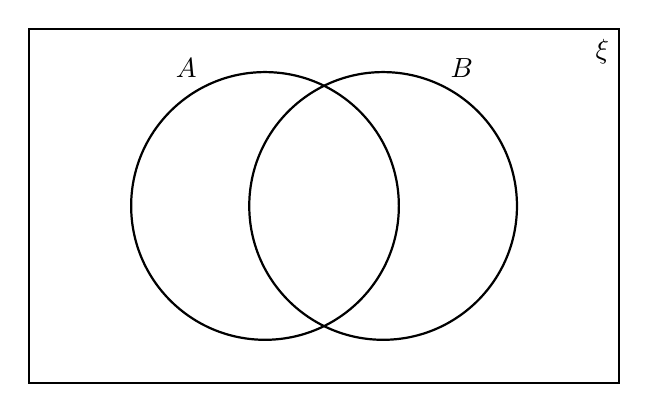
\begin{tikzpicture}[thick]
\draw (0,0) rectangle (7.5,4.5) node[anchor=north east] {$\xi$};
\draw (3,2.25) circle (1.7cm) node[above,shift={(-1,1.5)}] {$A$};
\draw (4.5,2.25) circle (1.7cm) node[above,shift={(1,1.5)}] {$B$};
\end{tikzpicture}
\end{center}
\[A\cup B = (A\cap \bar{B})\cup(A\cap B)\cup(\bar{A}\cap B)\]

Consider,\quad \quad \(B = (A\cap B)\cup(\bar{A}\cap B)\)
\[P(B) = P((A\cap B)\cup(\bar{A}\cap B)) \tag*{[Mutually Exclusive]}\]
\begin{equation}
P(B) = P(A\cap B)\cup P(\bar{A}\cap B) \label{eq:2}
\end{equation}

Consider,\quad \quad \(A = (A\cap B)\cup(A\cap \bar{B})\)
\[P(B) = P((A\cap B)\cup(A\cap \bar{B})) \tag*{[Mutually Exclusive]}\]
\begin{equation}
P(B) = P(A\cap B)\cup P(A\cap \bar{B}) \label{eq:3}
\end{equation}

Thus from \eqref{eq:2} and \eqref{eq:3} we get,
\begin{center}
\fbox{\(P(A\cup B)=P(A)+P(B)-P(A\cap B)\)}
\end{center}
\end{subequations}
\end{proof}

% = = = = = = GENERALISED ADDITION RULE = = = = = =
\subsection*{Generalised Addition Rule}

If $A_1,A_2,A_3\dots A_n$ are n events in a given sample space $S$.

\fbox{$ P(\bigcup\limits_{i=1}^n A_i) = \sum\limits_{i=1}^n P(A_i)\, - \,\sum\limits_{i=1}^n P(A_i\bigcap A_j) \, \dots \,(-1)^n\, P(\bigcap\sum\limits_{i=1}^n A_i) $}

% = = = = = = CONDITIONAL PROBABILITY = = = = = =
\subsection{Condtional Probability}
Conditional Probaility defines the probability of an event $\mathbb{A}$ under a given circumstance say $\mathbb{B}$ as follows:

\[P(A|B) = \frac{P(A\cap B)}{P(B)}\]

If the event is independent of the circumstance, then:

\[P(A)\cap B) = P(A) \times P(B)\]

% = = = = = = TOTAL PROBABILITY THEOREM = = = = = =
\subsection*{Total Probability Theorem}

If $B_1,B_2,B_3\dots B_k$ are partitions of S with $P(B_i) \neq 0$ \& $A$ is an arbitrary event of $S$, then

% \begin{equation*}
\fbox{$ P(A) = \sum\limits_{i=1}^k P(A|B_i)\times P(B_i) $}
% \end{equation*}

% = = = = = = PARTITIONS & BAYES THEROREM = = = = = = -
\subsection{Bayes' Theorem}
Let $B_1,B_2,B_3\dots B_k$ be events of S and are said to be partitions of S if:

\begin{itemize}
\item $\bigcup\limits_{i=1}^k B_i = S$
\item $B_i \cup B_j = \phi$
\end{itemize}

\underline{Bayes' Theorem}: 

If $B_1,B_2,B_3\dots B_k$ are partitions of S with $P(B_i) \neq 0$ \& $A$ is an arbitrary event of $S$, then

\begin{equation*}
P(B_i|A) = \frac{P(A|B_i)\times P(B_i)}{\sum\limits_{i=1}^k P(A|B_i)\times P(B_i)}
\end{equation*}
\end{document}